\documentclass[a4paper,12pt]{article}

\usepackage[utf8]{inputenc}
\usepackage[spanish]{babel}
\usepackage{amsmath, amssymb}
\usepackage{graphicx}
\usepackage{float}
\usepackage{booktabs}
\usepackage{xcolor}
\usepackage{listings}
\usepackage{caption}
\usepackage{fancyhdr}
\usepackage{hyperref}
\usepackage{tikz}

\hypersetup{
    colorlinks=true,
    linkcolor=blue,
    urlcolor=blue,
    pdftitle={Práctica 2 - Protocolo CAN},
}

% === Definición de colores similares a Vivado ===
\definecolor{vivadoKeyword}{rgb}{0.6,0.0,0.6}
\definecolor{vivadoComment}{rgb}{0.0,0.5,0.0}
\definecolor{vivadoString}{rgb}{0.5,0.2,0.0}
\definecolor{vivadoBackground}{rgb}{0.97,0.97,0.97}

\lstdefinelanguage{VHDL}{
    morekeywords={library, use, entity, is, port, in, out, end, architecture, of, begin, signal, if, then, else, when, others, xor, and, or, not},
    sensitive=true,
    morecomment=[l]--,
    morestring=[b]",
}

\lstset{
    language=VHDL,
    backgroundcolor=\color{vivadoBackground},
    keywordstyle=\color{vivadoKeyword}\bfseries,
    commentstyle=\color{vivadoComment}\itshape,
    stringstyle=\color{vivadoString},
    basicstyle=\ttfamily\small,
    numbers=left,
    numberstyle=\tiny,
    numbersep=5pt,
    frame=single,
    breaklines=true,
    tabsize=2,
    captionpos=b
}

\title{Práctica N°2: Medicion de Corriente con ajuste de PWM visualizado en OLED mediante comunicación Maestro-Esclavo con protocolo CAN}
\date{}

\begin{document}
\maketitle
\tableofcontents
\newpage


\section{Objetivos}

\subsection{Objetivo general}
Diseñar, implementar y validar una arquitectura maestro--esclavo basada en comunicación \textbf{CAN} sobre la plataforma \textit{STM32F407G-DISC1}, en la que el \textbf{maestro} mida en tiempo real la corriente del motor mediante un sensor Hall y la publique por CAN, mientras que el \textbf{esclavo} reciba dichos datos para visualizarlos en una pantalla OLED y actúe sobre el driver de motor mediante control PWM; adicionalmente, habilitar en el maestro una interfaz por \textbf{UART2} para telemetría y para el envío de comandos de control (\texttt{A/a} para incrementar y \texttt{d/D} para decrementar el PWM del motor del esclavo).

\subsection{Objetivos específicos}
\begin{itemize}
  \item \textbf{Configurar el bus CAN} del STM32 (bit timing, modo normal/loopback para pruebas, filtros de aceptación e IDs) y definir un \emph{frame set} mínimo (IDs, frecuencia de publicación y formato de payload) para corriente, estado y comandos.
  \item \textbf{Adquirir y escalar la corriente} en el maestro desde el sensor Hall (vía SPI u otra interfaz según el módulo empleado), implementando linealización, conversión a unidades físicas (A) y verificación básica de rango.
  \item \textbf{Implementar telemetría por UART2} en el maestro para imprimir corriente, estado del sistema y confirmaciones de comandos; mapear los caracteres \texttt{A/a} y \texttt{d/D} a mensajes CAN de “\emph{incremento/decremento de PWM}”.
  \item \textbf{Recibir y procesar tramas CAN} en el esclavo para actualizar el \emph{setpoint} de PWM del motor y mantener sincronizado el estado mostrado en la pantalla.
  \item \textbf{Controlar el motor por PWM} en el esclavo (TIM adecuado) mediante el driver \emph{TB6549FG} u otro equivalente, garantizando una resolución y frecuencia de conmutación apropiadas para la aplicación.
  \item \textbf{Visualizar en OLED} (p.\,ej., SSD1351) en el esclavo las magnitudes relevantes: corriente instantánea, porcentaje de PWM, ID/estado del bus, y mensajes de alerta.
  \item \textbf{Robustecer la comunicación}: manejo de errores CAN (TEC/REC, \emph{error frames}), reintentos y estados \emph{bus-off}; validaciones de integridad de payload y \emph{timeouts} en el esclavo ante pérdida de telegramas.
  \item \textbf{Seguridad funcional básica}: límites de PWM y corriente (clamp y/o apagado) para proteger el motor y la electrónica ante sobrecorriente o comandos inválidos.
  \item \textbf{Plan de pruebas y métricas}: verificar latencia extremo a extremo (medición UART$\rightarrow$CAN$\rightarrow$PWM), tasa de actualización, ocupación del bus y comportamiento ante fallos (desconexión del maestro, ruido, colisiones).
  \item \textbf{Documentación reproducible}: registrar mapeos de pines, parámetros de CAN, esquema de IDs, formato de tramas, versiones de firmware y pasos de compilación/descarga para facilitar replicación en laboratorio.
\end{itemize}

\section{Guía de configuración del Maestro en STM32CubeMX (\texttt{.ioc})}

\subsection{Pines en el ioc}
% Reemplaza las rutas por tus fotos reales
\begin{figure}[H]
  \centering
  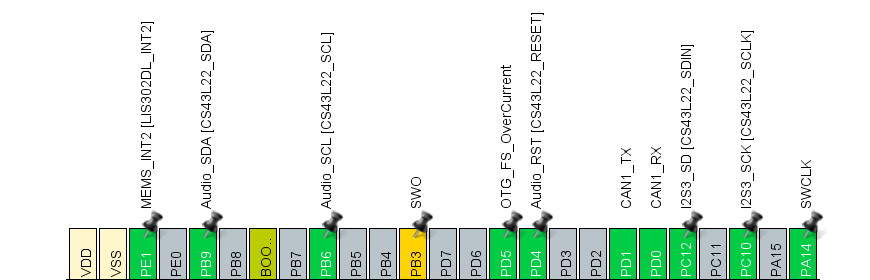
\includegraphics[width=.95\textwidth]{ioc_maestro/norte_maestro.png}
  \caption{Vista superior (lado norte) del STM32F407G-DISC1 del maestro.}
  \label{fig:maestro_lado_norte}
\end{figure}

\begin{figure}[H]
  \centering
  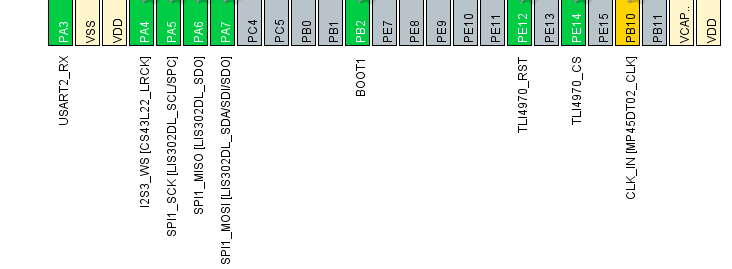
\includegraphics[width=.95\textwidth]{ioc_maestro/sur_maestro.png}
  \caption{Vista inferior (lado sur).}
  \label{fig:maestro_lado_sur}
\end{figure}

\begin{figure}[H]
  \centering
  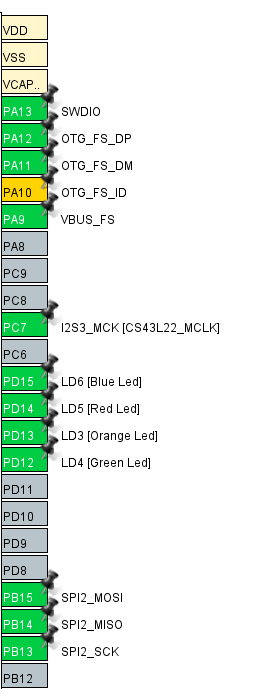
\includegraphics[angle=270,width=.75\textwidth]{ioc_maestro/este_maestro.png}
  \caption{Vista lateral (este). }
  \label{fig:maestro_lado_este}
\end{figure}

\begin{figure}[H]
  \centering
  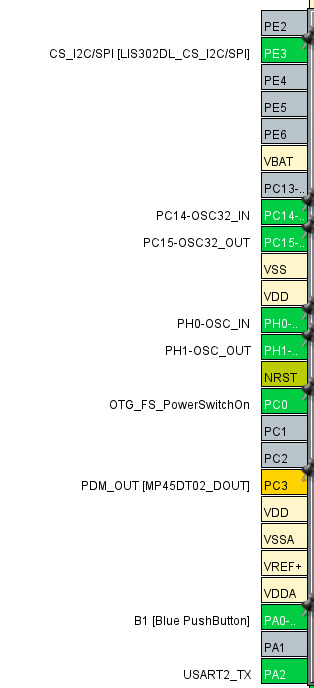
\includegraphics[angle=270,width=.75\textwidth]{ioc_maestro/oeste_maestro.png}
  \caption{Vista lateral (oeste).}
  \label{fig:maestro_lado_oeste}
\end{figure}

\begin{figure}[H]
  \centering
  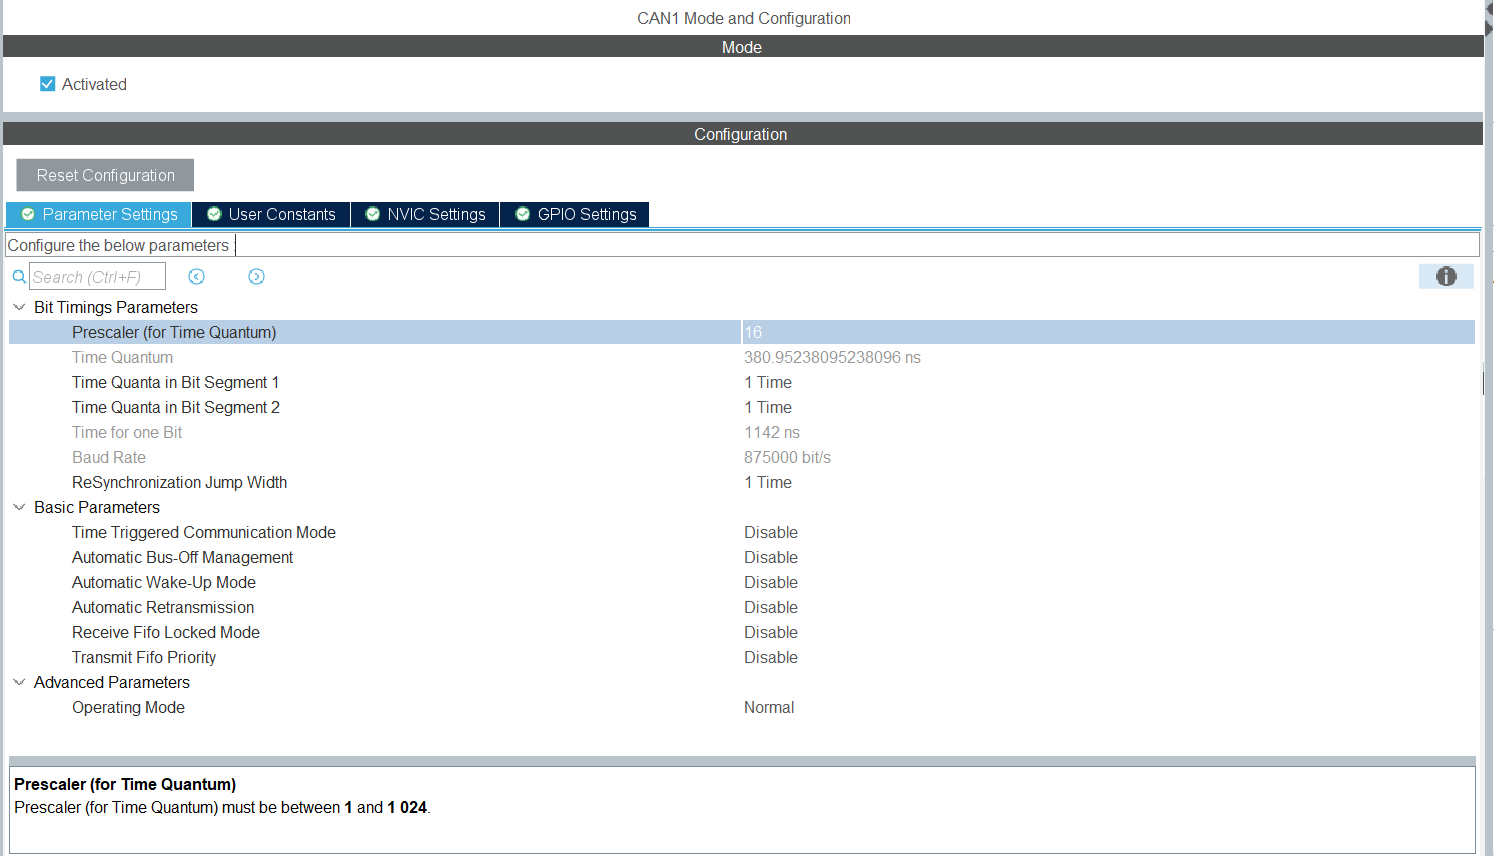
\includegraphics[width=.8\textwidth]{ioc_maestro/can1.png}
  \caption{STM32CubeMX: configuración de \textbf{CAN1} (modo Normal, temporización nominal)}
  \label{fig:ioc_can1}
\end{figure}

\begin{figure}[H]
  \centering
  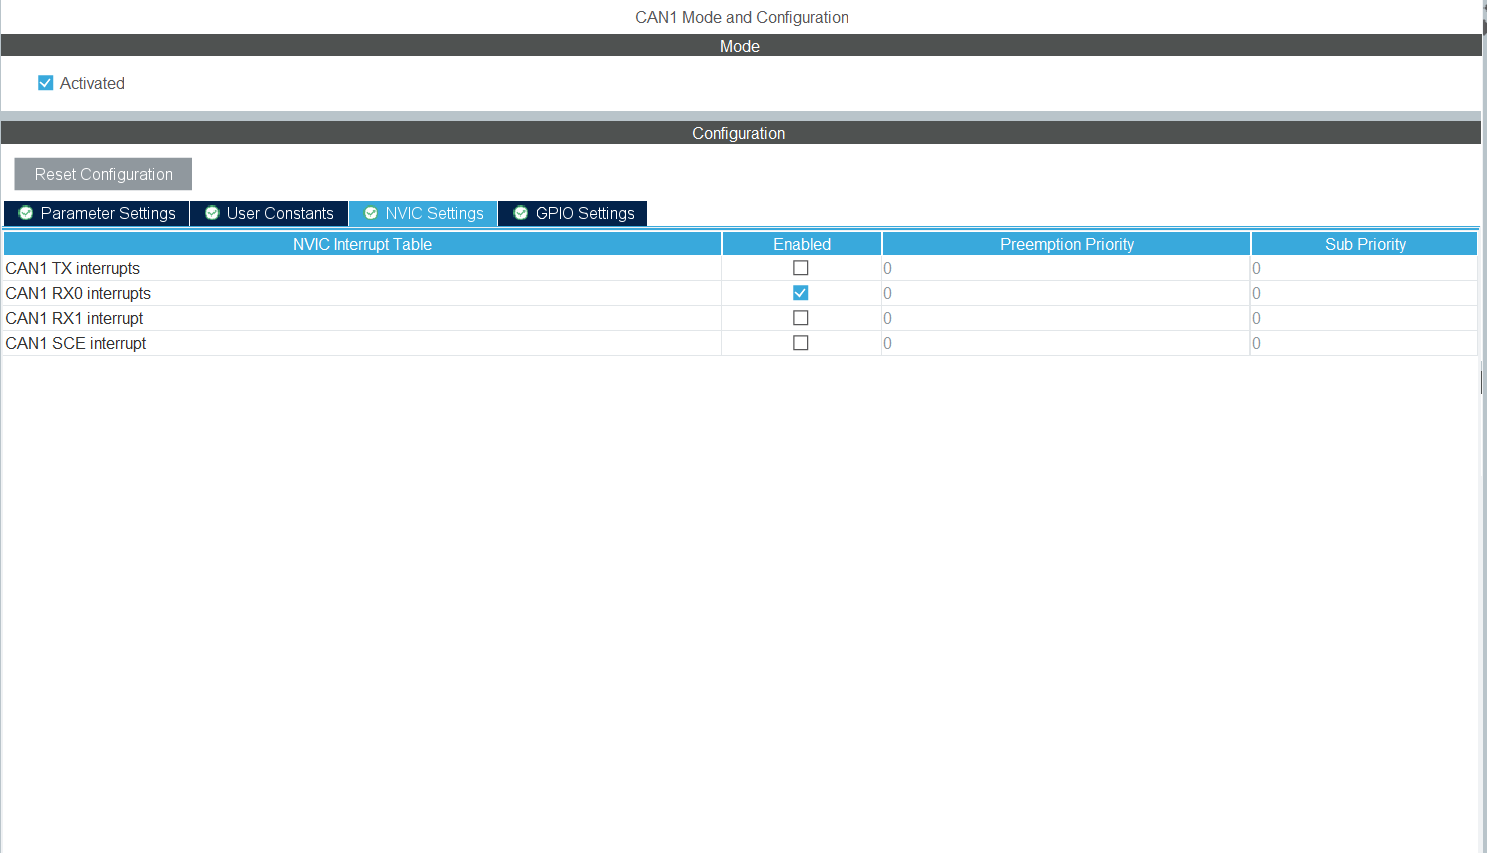
\includegraphics[width=.8\textwidth]{ioc_maestro/can2.png}
  \caption{STM32CubeMX: configuración de \textbf{CAN1} (modo Normal, temporización nominal)}
  \label{fig:ioc_can1}
\end{figure}

\begin{figure}[H]
  \centering
  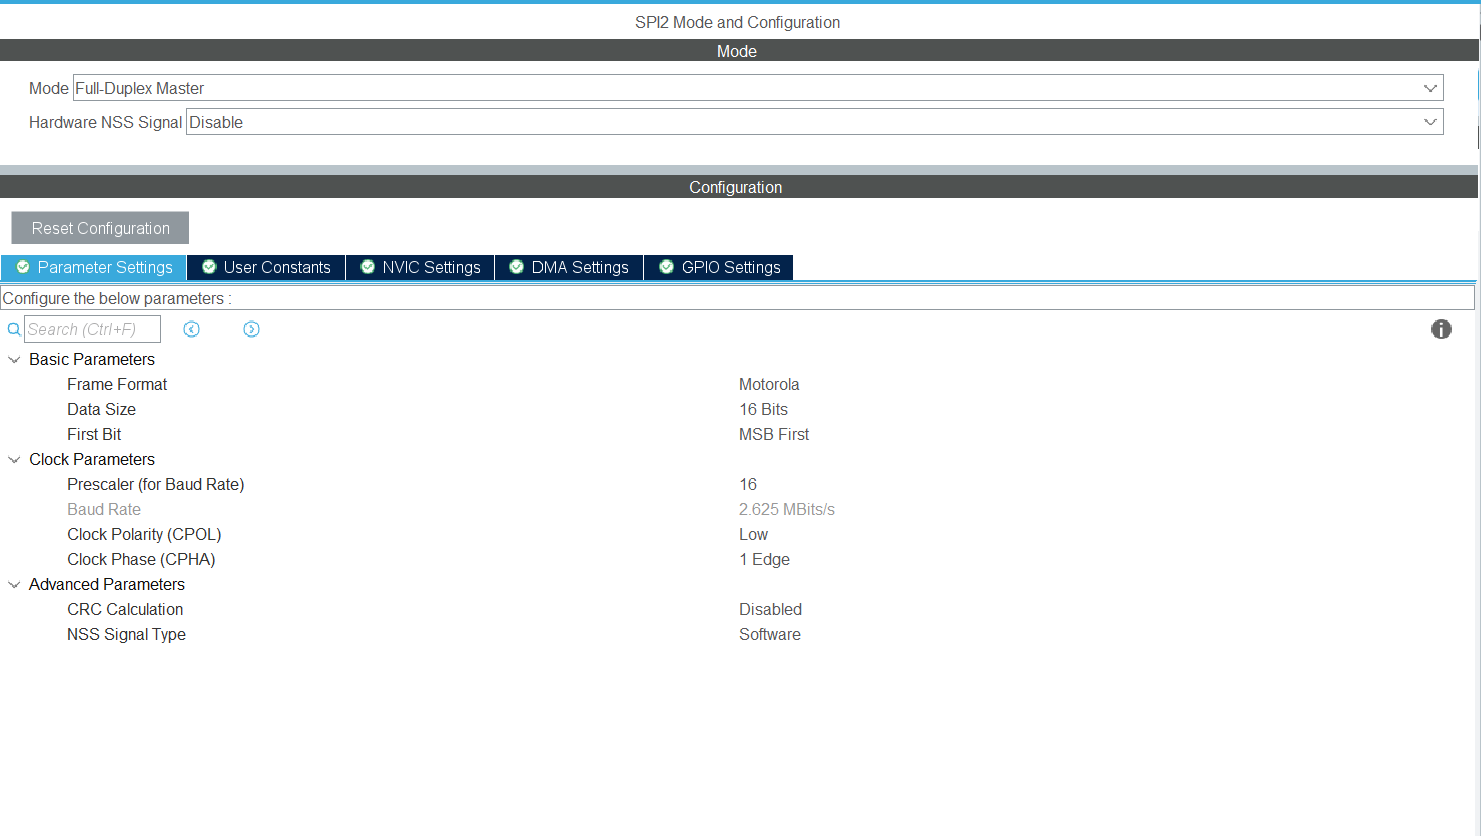
\includegraphics[width=.8\textwidth]{ioc_maestro/spi2.png}
  \caption{STM32CubeMX: \textbf{SPI2} en modo maestro.}
  \label{fig:ioc_spi2}
\end{figure}


\begin{figure}[H]
  \centering
  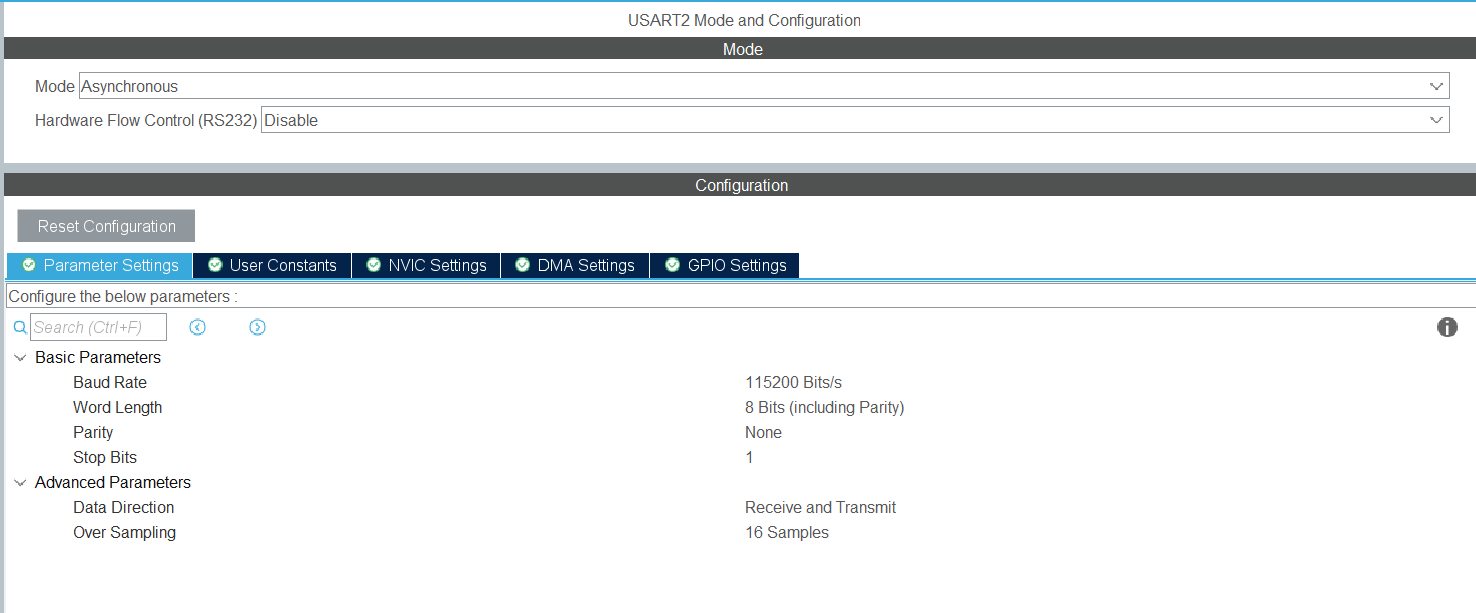
\includegraphics[width=.8\textwidth]{ioc_maestro/uart2.png}
  \caption{STM32CubeMX: \textbf{USART2}.}
  \label{fig:ioc_usart2}
\end{figure}

\begin{figure}[H]
  \centering
  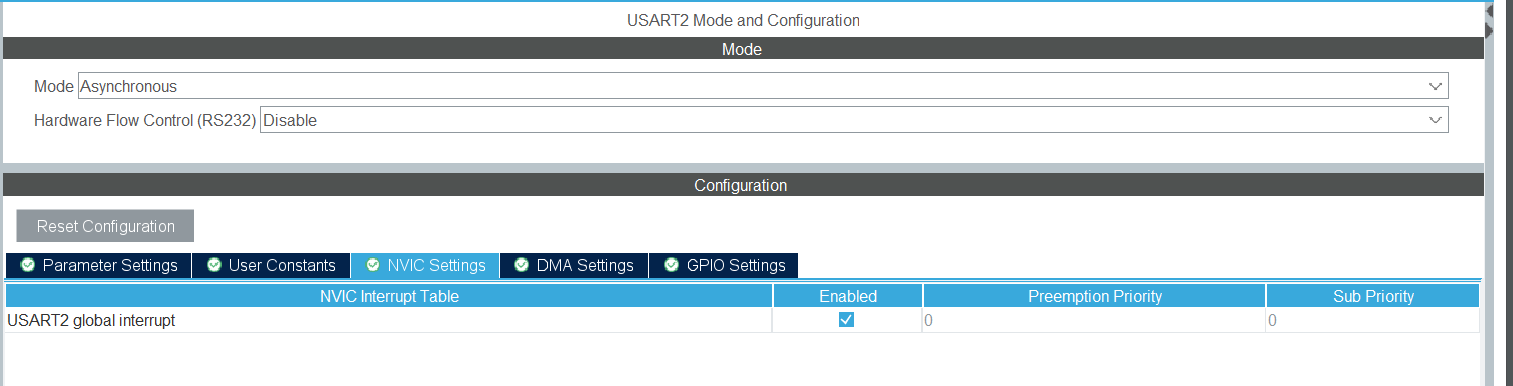
\includegraphics[width=.8\textwidth]{ioc_maestro/uart22.png}
  \caption{STM32CubeMX: \textbf{USART2}.}
  \label{fig:ioc_usart2}
\end{figure}

\begin{figure}[H]
  \centering
  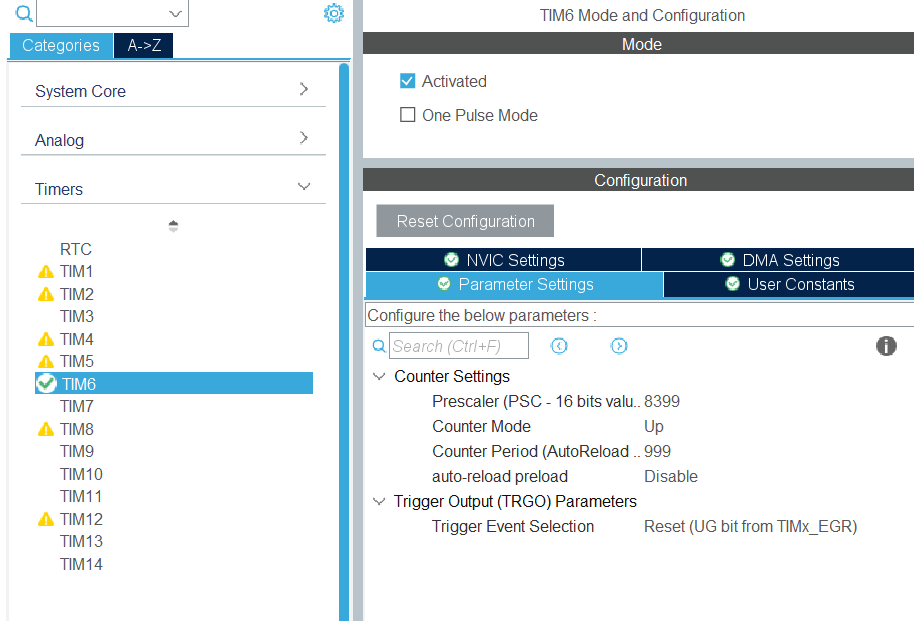
\includegraphics[width=.8\textwidth]{ioc_maestro/tim6.png}
  \caption{STM32CubeMX: \textbf{TIM6}.}
  \label{fig:ioc_usart2}
\end{figure}





% ================== USART2 ==================
\subsection{USART2 — Telemetría y comandos desde PC}
\textbf{Propósito:} imprimir corriente y leer las teclas \texttt{A/a} (subir PWM) y \texttt{D/d} (bajar PWM).

\paragraph{Configuración básica}
\begin{enumerate}
  \item Habilita \textbf{USART2}.
  \item Parámetros: \textbf{115200\,baud}, 8\,N\,1, sin control de flujo (\texttt{None}).
  \item \textbf{Modo}: TX y RX.
  \item En \textit{NVIC}, habilita la \textbf{interrupción de USART2} (para recepción por IT).
\end{enumerate}

\paragraph{Asignación de pines (AF7)}
\begin{itemize}
  \item \textbf{PA2} $\rightarrow$ USART2\_TX (AF7)
  \item \textbf{PA3} $\rightarrow$ USART2\_RX (AF7)
\end{itemize}



% ================== SPI2 + GPIO ==================
\subsection{SPI2 + GPIO — Sensor de corriente Hall (TLI4970)}
\textbf{Propósito:} adquirir la corriente del motor.

\paragraph{SPI2 (AF5)}
\begin{enumerate}
  \item Habilita \textbf{SPI2} como \textbf{Master}.
  \item Parámetros:
  \begin{itemize}
    \item \texttt{Data Size} = \textbf{16 bits}
    \item \texttt{CPOL} = Low, \texttt{CPHA} = 1Edge
    \item \texttt{NSS} = Software, \texttt{First Bit} = MSB
    \item \texttt{BaudRate Prescaler} = \textbf{16}
  \end{itemize}
  \item Pines:
  \begin{itemize}
    \item \textbf{PB13} = SPI2\_SCK (AF5)
    \item \textbf{PB14} = SPI2\_MISO (AF5)
    \item \textbf{PB15} = SPI2\_MOSI (AF5)
  \end{itemize}
\end{enumerate}

\paragraph{GPIO de control del sensor}
\begin{itemize}
  \item \textbf{PE5} = \texttt{TLI4970\_CS} $\rightarrow$ \textbf{GPIO Output} (Push--Pull, Low speed)
  \item \textbf{PE10} = \texttt{TLI4970\_RST} $\rightarrow$ \textbf{GPIO Output} (Push--Pull, Low speed)
\end{itemize}



% ================== TIM6 (opcional) ==================
\subsection{TIM6  — Base de tiempos estable}
\textbf{Propósito:} temporizar tareas periódicas (telemetría, publicación CAN) con jitter bajo.

\paragraph{Configuración sugerida}
\begin{itemize}
  \item \textbf{TIM6} como \textit{time base}. Prescaler y Period para \textbf{10\,Hz} (100\,ms por actualización).
  \item Habilita interrupción del TIM6 si quieres disparar tareas periódicas sin \texttt{HAL\_Delay}.
\end{itemize}

% (Opcional, colócalo en el preámbulo de tu documento)
\lstset{
  language=C,
  basicstyle=\ttfamily\small,
  keywordstyle=\bfseries,
  commentstyle=\itshape\color{gray},
  numbers=left, numberstyle=\tiny, numbersep=6pt,
  frame=single, breaklines=true, tabsize=2
}

\section{Explicación del código del Maestro}

\subsection{Includes}
\begin{lstlisting}
// HAL y middlewares generados
#include "main.h"
#include "usb_host.h"

// Librerías estándar C
#include <stdio.h>
#include <string.h>
\end{lstlisting}

\noindent\textbf{¿Para qué sirven?} 
\begin{itemize}
  \item \texttt{main.h} / \texttt{usb\_host.h}: definiciones del hardware y middlewares generados por CubeMX.
  \item \texttt{stdio.h} / \texttt{string.h}: formateo de textos (p.ej., \texttt{sprintf}) y manejo de buffers para UART.
\end{itemize}

\subsection{Variables globales y \textit{handles} de periféricos}
\begin{lstlisting}
// Handles de periféricos (HAL)
CAN_HandleTypeDef hcan1;

I2C_HandleTypeDef hi2c1;
I2S_HandleTypeDef hi2s3;

SPI_HandleTypeDef hspi1;
SPI_HandleTypeDef hspi2;

TIM_HandleTypeDef htim6;

UART_HandleTypeDef huart2;

// Variables de aplicación
uint8_t uart_rx_data;                  // Byte recibido por UART2
volatile uint8_t motor_duty_cycle = 0; // Consigna de PWM (0..100%)
\end{lstlisting}

\newpage
\noindent\textbf{Idea clave.}
\begin{itemize}
  \item Los \textit{handles} encapsulan el estado de cada periférico; se pasan a las funciones HAL.
  \item \texttt{uart\_rx\_data} es un buffer de 1 byte para comandos.
  \item \texttt{motor\_duty\_cycle} es \texttt{volatile} porque puede cambiar dentro de una interrupción.
\end{itemize}

\subsection{Prototipos de funciones de inicialización}
\begin{lstlisting}
void SystemClock_Config(void);
static void MX_GPIO_Init(void);
static void MX_I2C1_Init(void);
static void MX_I2S3_Init(void);
static void MX_SPI1_Init(void);
static void MX_CAN1_Init(void);
static void MX_SPI2_Init(void);
static void MX_TIM6_Init(void);
static void MX_USART2_UART_Init(void);
void MX_USB_HOST_Process(void);
\end{lstlisting}

\noindent\textbf{Lectura guiada.} Cada \texttt{MX\_\ldots\_Init} prepara un periférico (modo, pines, velocidades, IRQ). En esta práctica nos interesan especialmente \textbf{CAN1}, \textbf{SPI2} (sensor Hall) y \textbf{USART2} (telemetría/comandos). \textbf{TIM6} es útil si luego quieres periodicidad precisa sin \texttt{HAL\_Delay}.

\newpage

\subsection{Callback por interrupción de UART (recepción de comandos)}
\begin{lstlisting}
void HAL_UART_RxCpltCallback(UART_HandleTypeDef *huart)
{
  if (huart->Instance == USART2)
  {
    if (uart_rx_data == 'A' || uart_rx_data == 'a') {
      if (motor_duty_cycle <= 95) motor_duty_cycle += 5;
      else motor_duty_cycle = 100;
    }
    else if (uart_rx_data == 'D' || uart_rx_data == 'd') {
      if (motor_duty_cycle >= 5) motor_duty_cycle -= 5;
      else motor_duty_cycle = 0;
    }

    // Feedback por UART
    char command_buf[60];
    sprintf(command_buf, "Comando: %s. Nueva velocidad objetivo: %d%%\r\n",
            (uart_rx_data == 'A' || uart_rx_data == 'a') ? "Aumentar" : "Disminuir",
            motor_duty_cycle);
    HAL_UART_Transmit(&huart2, (uint8_t*)command_buf, strlen(command_buf), 100);

    // Publicar consigna por CAN (ID 0x124, DLC=1)
    CAN_TxHeaderTypeDef TxHeader;
    uint32_t TxMailbox;
    uint8_t speed_data[1] = { motor_duty_cycle };
    TxHeader.StdId = 0x124;
    TxHeader.RTR   = CAN_RTR_DATA;
    TxHeader.IDE   = CAN_ID_STD;
    TxHeader.DLC   = 1;
    HAL_CAN_AddTxMessage(&hcan1, &TxHeader, speed_data, &TxMailbox);

    // Re-armar la recepción por interrupción (escuchar el siguiente byte)
    HAL_UART_Receive_IT(&huart2, &uart_rx_data, 1);
  }
}
\end{lstlisting}

\noindent\textbf{Puntos importantes.}
\begin{itemize}
  \item El callback se ejecuta cuando llega \textbf{un byte} por \textbf{USART2}.
  \item Mapa de comandos: \texttt{A/a} $\rightarrow$ +5\%, \texttt{D/d} $\rightarrow$  $-5$ \% (saturado a [0,100]).
  \item Se informa por UART y se envía la nueva consigna por CAN (ID \texttt{0x124}).
  \item \underline{Crítico:} volver a llamar a \texttt{HAL\_UART\_Receive\_IT} para seguir recibiendo.
\end{itemize}

\subsection{\texttt{main()} — Secuencia de arranque y lazo principal}
\begin{lstlisting}
int main(void)
{
  /* Reset de HAL y SysTick */
  HAL_Init();

  /* Árbol de relojes del sistema */
  SystemClock_Config();

  /* Inicialización de periféricos */
  MX_GPIO_Init();
  MX_I2C1_Init();
  MX_I2S3_Init();
  MX_SPI1_Init();
  MX_USB_HOST_Init();
  MX_CAN1_Init();
  MX_SPI2_Init();
  MX_TIM6_Init();
  MX_USART2_UART_Init();

  /* UART2: recibir por interrupción (1 byte) */
  HAL_UART_Receive_IT(&huart2, &uart_rx_data, 1);

  /* CAN1: arrancar el bus */
  if (HAL_CAN_Start(&hcan1) != HAL_OK) {
      Error_Handler();
  }

  /* Bucle principal */
  while (1)
  {
    MX_USB_HOST_Process();  // No interfiere si no usas USB

    /* --- Adquisición y filtrado de corriente (SPI2) --- */
    const int NUM_SAMPLES = 100;
    int32_t sum_current_value = 0;

    for (int i = 0; i < NUM_SAMPLES; i++) {
        uint16_t raw_spi_frame = 0;

        // Control manual de CS (GPIO)
        HAL_GPIO_WritePin(TLI4970_CS_GPIO_Port, TLI4970_CS_Pin, GPIO_PIN_RESET);
        HAL_Delay(1);
        HAL_SPI_Receive(&hspi2, (uint8_t *)&raw_spi_frame, 1, 100);
        HAL_GPIO_WritePin(TLI4970_CS_GPIO_Port, TLI4970_CS_Pin, GPIO_PIN_SET);

        // Swap de bytes (endianness)
        raw_spi_frame = (raw_spi_frame << 8) | (raw_spi_frame >> 8);

        // Extraer 13 bits con signo + extensión de signo
        int16_t current_value_13bit = raw_spi_frame & 0x1FFF;
        if (current_value_13bit & 0x1000) {
            current_value_13bit |= 0xE000;
        }

        sum_current_value += current_value_13bit;
    }

    // Promedio y escala a miliamperios (12.5 mA/LSB)
    float current_mA = (float)(sum_current_value / NUM_SAMPLES) * 12.5f;

    /* --- Transmisión por CAN: corriente (ID 0x123, 2 bytes big-endian) --- */
    CAN_TxHeaderTypeDef TxHeader;
    uint32_t TxMailbox;
    uint8_t can_data[2];
    TxHeader.StdId = 0x123;
    TxHeader.RTR   = CAN_RTR_DATA;
    TxHeader.IDE   = CAN_ID_STD;
    TxHeader.DLC   = 2;

    int16_t current_to_send = (int16_t)current_mA;
    can_data[0] = (uint8_t)(current_to_send >> 8);
    can_data[1] = (uint8_t)(current_to_send);
    HAL_CAN_AddTxMessage(&hcan1, &TxHeader, can_data, &TxMailbox);

    /* --- Telemetría UART --- */
    char uart_buf[50];
    sprintf(uart_buf, "Corriente: %.2f mA\r\n", current_mA);
    HAL_UART_Transmit(&huart2, (uint8_t*)uart_buf, strlen(uart_buf), 100);

    /* Periodicidad simple (0.5 s). Mejora futura: TIM6 + IRQ */
    HAL_Delay(500);
  }
}
\end{lstlisting}

\noindent\textbf{Cómo leer este flujo.}
\begin{enumerate}
  \item Arranque de HAL y relojes; luego inicialización de periféricos.
  \item Se habilita la recepción por interrupción en UART2 y se pone CAN1 operativo.
  \item En el \texttt{while(1)}:
    \begin{enumerate}
      \item Se adquieren 100 muestras por SPI2 con control manual de CS y corrección de \emph{endianness}.
      \item Se extraen 13 bits con signo, se promedian y se escalan a mA.
      \item Se envía la corriente por CAN (ID \texttt{0x123}) y se imprime por UART.
      \item Se espera 500 ms (versión simple y entendible para iniciar).
    \end{enumerate}
\end{enumerate}

\newpage

\section{Configuración del Esclavo en STM32CubeMX (\texttt{.ioc})}

% ===========================
% FOTOS DE LA PLACA (4 LADOS)
% ===========================
\begin{figure}[H]
  \centering
  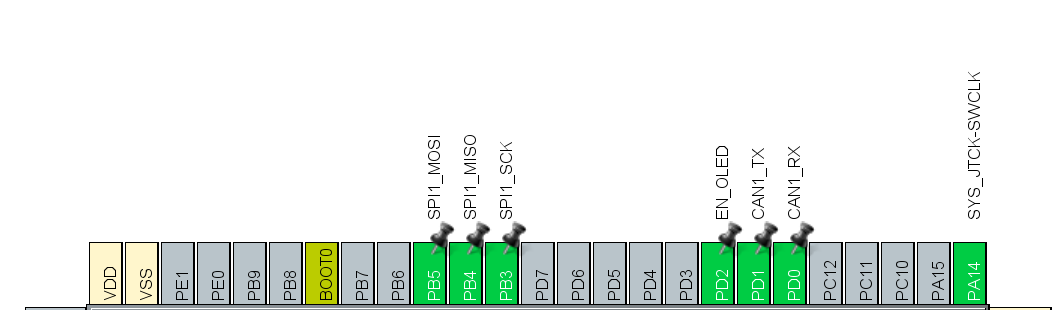
\includegraphics[width=.95\textwidth]{ioc_esclavo/norte_esclavo.png}
  \caption{Esclavo — vista superior (lado norte).}
  \label{fig:esclavo_lado_norte}
\end{figure}

\begin{figure}[H]
  \centering
  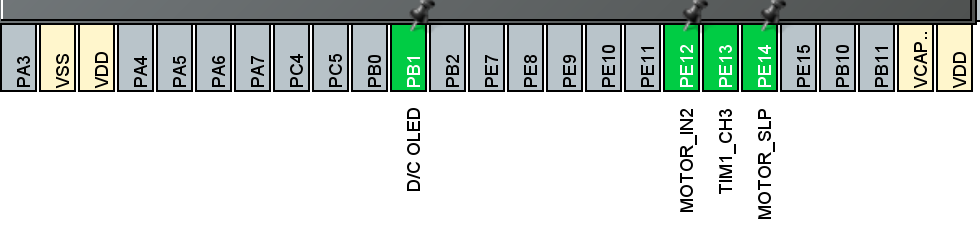
\includegraphics[width=.95\textwidth]{ioc_esclavo/sur_esclavo.png}
  \caption{Esclavo — vista inferior (lado sur).}
  \label{fig:esclavo_lado_sur}
\end{figure}

\begin{figure}[H]
  \centering
  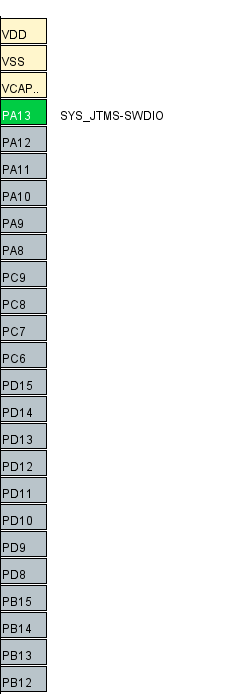
\includegraphics[angle=270,width=.95\textwidth]{ioc_esclavo/este_esclavo.png}
  \caption{Esclavo — vista lateral (este).}
  \label{fig:esclavo_lado_este}
\end{figure}

\begin{figure}[H]
  \centering
  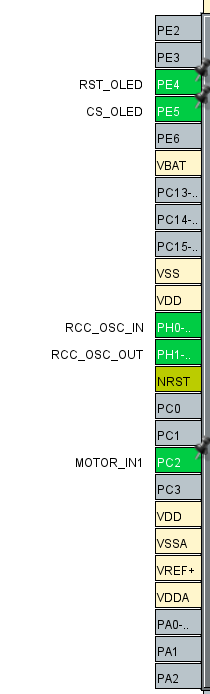
\includegraphics[angle=270,width=.95\textwidth]{ioc_esclavo/oeste_esclavo.png}
  \caption{Esclavo — vista lateral (oeste)s.}
  \label{fig:esclavo_lado_oeste}
\end{figure}

% ==========================================
% CAPTURAS DEL IOC (PERIFÉRICOS POR SEPARADO)
% ==========================================

% CAN1
\begin{figure}[H]
  \centering
  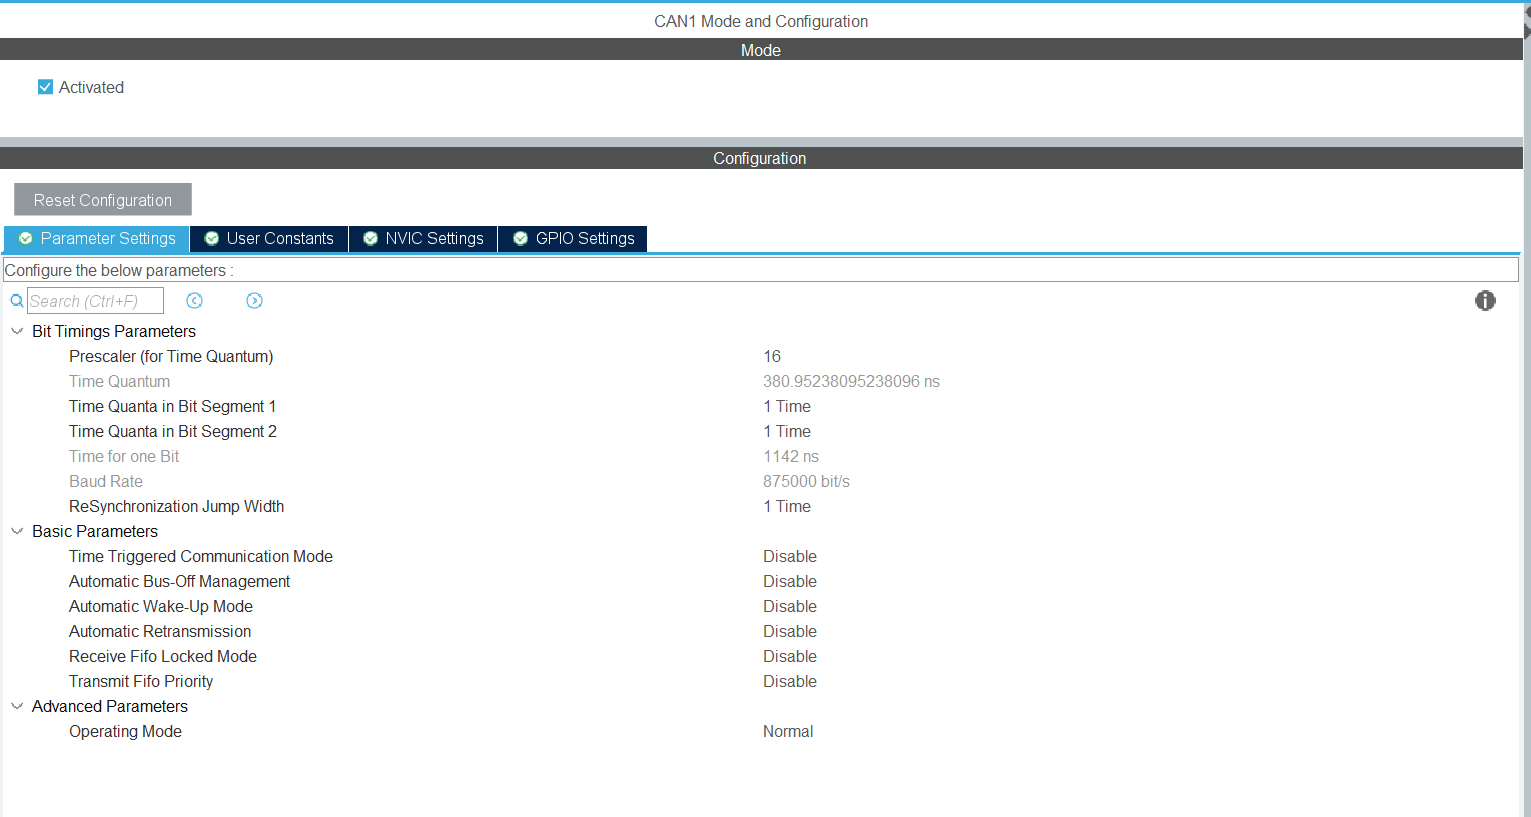
\includegraphics[width=.82\textwidth]{ioc_esclavo/can1.png}
  \caption{STM32CubeMX — Esclavo: configuración de \textbf{CAN1} en modo normal, filtros y notificaciones de recepción activas.}
  \label{fig:ioc_esclavo_can1}
\end{figure}

\begin{figure}[H]
  \centering
  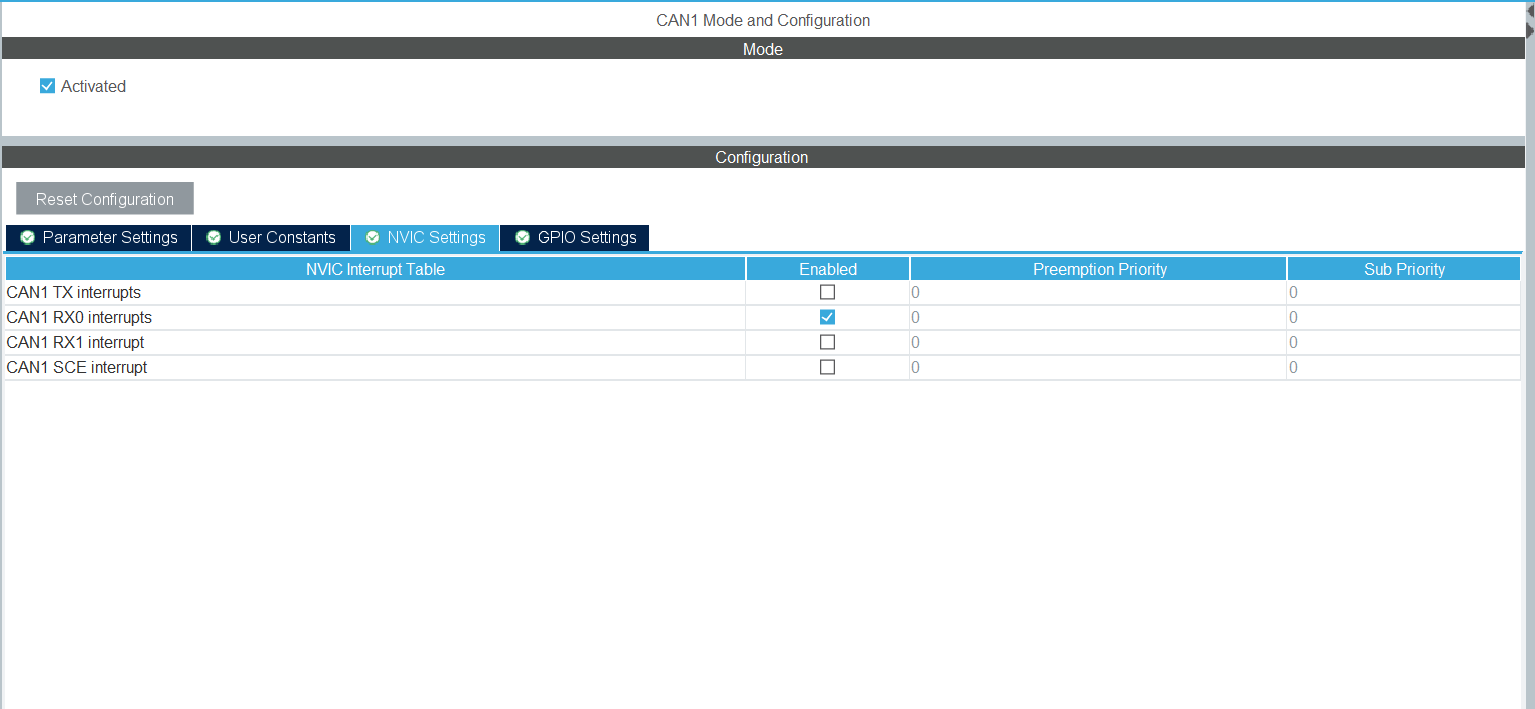
\includegraphics[width=.82\textwidth]{ioc_esclavo/can2.png}
  \caption{STM32CubeMX — Esclavo: configuración de \textbf{CAN1} en modo normal, filtros y notificaciones de recepción activas.}
  \label{fig:ioc_esclavo_can1}
\end{figure}



% SPI1 (OLED)
\begin{figure}[H]
  \centering
  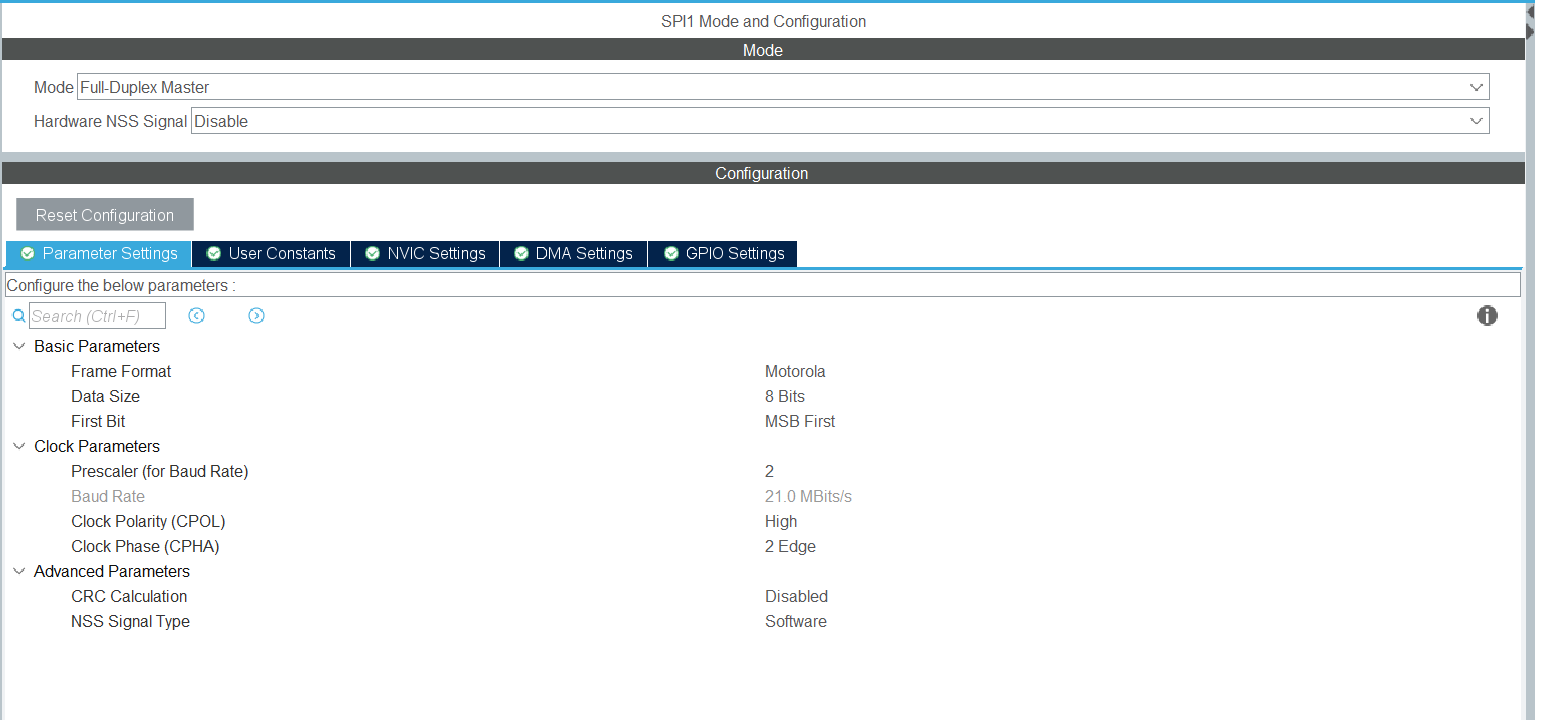
\includegraphics[width=.82\textwidth]{ioc_esclavo/sp11.png}
  \caption{STM32CubeMX — Esclavo: \textbf{SPI1} configurado para la \textbf{OLED SSD1351}. Ajustes de modo maestro y parámetros de transferencia.}
  \label{fig:ioc_esclavo_spi1}
\end{figure}

% TIM1 (PWM motor)
\begin{figure}[H]
  \centering
  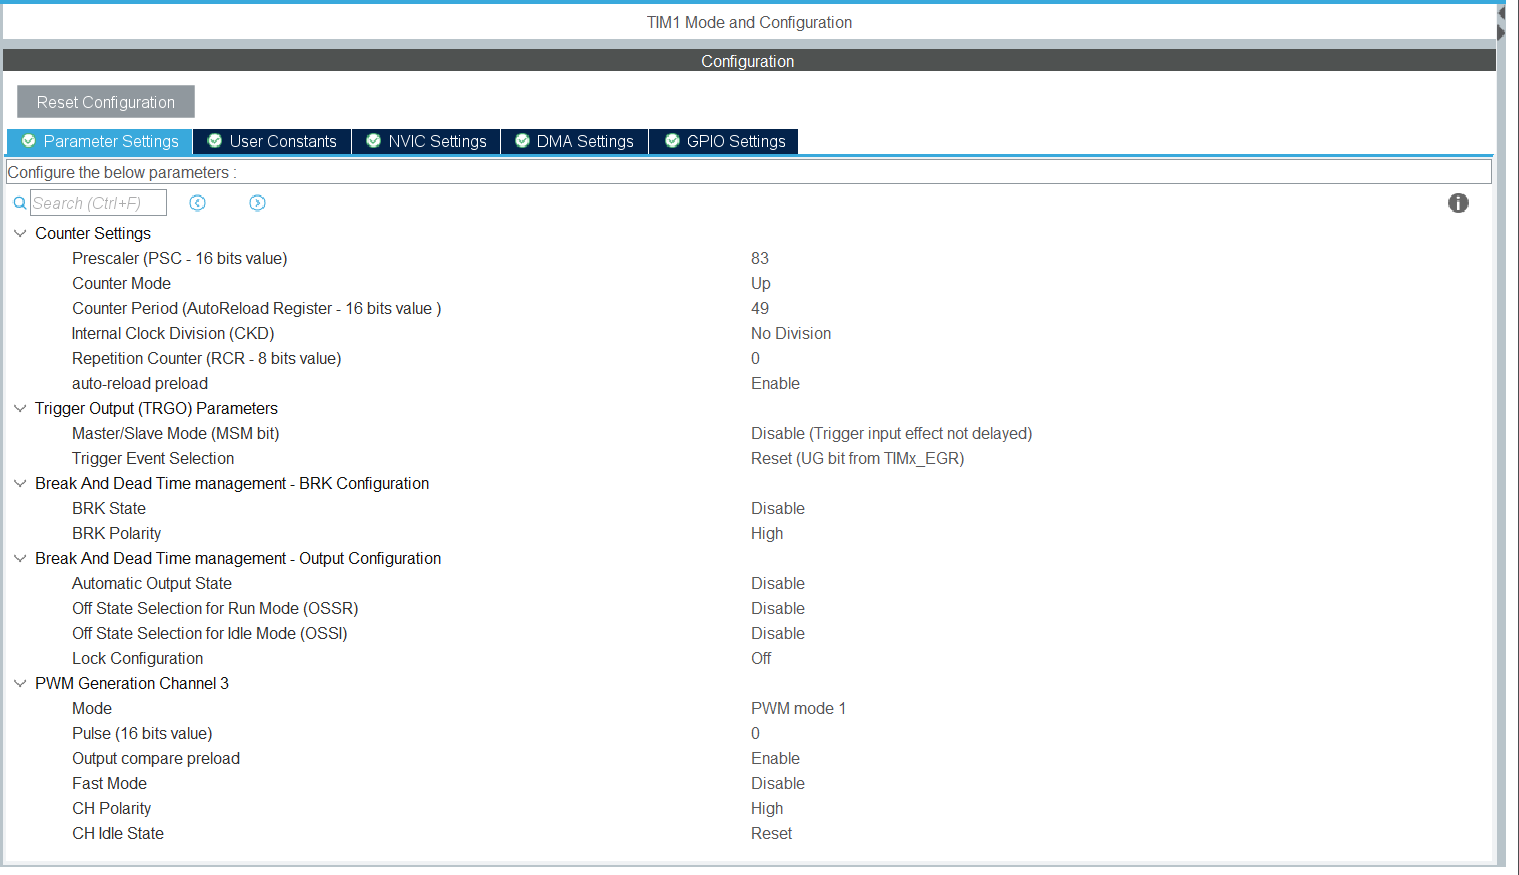
\includegraphics[width=.82\textwidth]{ioc_esclavo/tim1.png}
  \caption{STM32CubeMX — Esclavo: \textbf{TIM1} en \textbf{PWM} para el control de velocidad del motor mediante el driver.}
  \label{fig:ioc_esclavo_tim1_pwm}
\end{figure}

\newpage

\section{Explicación del código del Esclavo}



\subsection{Macros y constantes de aplicación}
\begin{lstlisting}
/* USER CODE BEGIN PD */
#define CAN_ID_CURRENT 0x123
#define CAN_ID_SPEED   0x124

#define BLACK   0x0000
#define WHITE   0xFFFF
#define RED     0xF800
#define GREEN   0x07E0
#define BLUE    0x001F
#define YELLOW  0xFFE0
/* USER CODE END PD */
\end{lstlisting}

\noindent\textbf{Lectura guiada.}
\begin{itemize}
  \item \texttt{CAN\_ID\_CURRENT} y \texttt{CAN\_ID\_SPEED}: identificadores de las tramas que el nodo debe aceptar (corriente y consigna de velocidad).
  \item Constantes de color para la OLED (formato RGB565): facilitan textos legibles y consistentes.
\end{itemize}

\subsection{Variables globales y \textit{handles}}
\begin{lstlisting}
/* Private variables -------------------------------------*/
CAN_HandleTypeDef hcan1;

SPI_HandleTypeDef hspi1;

TIM_HandleTypeDef htim1;

/* USER CODE BEGIN PV */
volatile int16_t g_current_mA = 0;
volatile uint8_t g_motor_speed_percent = 0;
volatile _Bool g_update_display_flag = 0;
/* USER CODE END PV */
\end{lstlisting}

\noindent\textbf{Puntos importantes.}
\begin{itemize}
  \item \textbf{Estado de periféricos}: \texttt{hcan1}, \texttt{hspi1} (OLED), \texttt{htim1} (PWM motor).
  \item \textbf{Volátiles}: las variables compartidas con interrupciones (\texttt{g\_current\_mA}, \texttt{g\_motor\_speed\_percent}, \texttt{g\_update\_display\_flag}) son \texttt{volatile} para evitar que el compilador “optimice” lecturas/escrituras asíncronas.
\end{itemize}

\subsection{Prototipos relevantes}
\begin{lstlisting}
void SystemClock_Config(void);
static void MX_GPIO_Init(void);
static void MX_CAN1_Init(void);
static void MX_SPI1_Init(void);
static void MX_TIM1_Init(void);
/* USER CODE BEGIN PFP */
void Update_OLED_Display(void);
static void CAN_Filter_Config(void);
/* USER CODE END PFP */
\end{lstlisting}

\noindent\textbf{Idea clave.}
\begin{itemize}
  \item Las funciones \texttt{MX\_\ldots\_Init} inicializan periféricos.
  \item \texttt{CAN\_Filter\_Config}: configura filtros para recibir \textbf{solo} lo que interesa (IDs de corriente y velocidad).
  \item \texttt{Update\_OLED\_Display}: encapsula la lógica de refresco de pantalla para no mezclarla con las ISR.
\end{itemize}

\subsection{Configuración de filtros CAN y callback de recepción}
\begin{lstlisting}
/* USER CODE BEGIN 4 */
static void CAN_Filter_Config(void)
{
  CAN_FilterTypeDef canfilterconfig;
  canfilterconfig.FilterActivation     = CAN_FILTER_ENABLE;
  canfilterconfig.FilterBank           = 0;
  canfilterconfig.FilterFIFOAssignment = CAN_RX_FIFO0;
  canfilterconfig.FilterMode           = CAN_FILTERMODE_IDLIST;
  canfilterconfig.FilterScale          = CAN_FILTERSCALE_32BIT;
  canfilterconfig.SlaveStartFilterBank = 14;
  canfilterconfig.FilterIdHigh         = CAN_ID_CURRENT << 5;
  canfilterconfig.FilterIdLow          = 0x0000;
  canfilterconfig.FilterMaskIdHigh     = CAN_ID_SPEED << 5;
  canfilterconfig.FilterMaskIdLow      = 0x0000;
  if(HAL_CAN_ConfigFilter(&hcan1, &canfilterconfig) != HAL_OK) { Error_Handler(); }
}

void HAL_CAN_RxFifo0MsgPendingCallback(CAN_HandleTypeDef *hcan)
{
    CAN_RxHeaderTypeDef RxHeader;
    uint8_t RxData[8];
    if (HAL_CAN_GetRxMessage(hcan, CAN_RX_FIFO0, &RxHeader, RxData) == HAL_OK)
    {
        if (RxHeader.StdId == CAN_ID_CURRENT && RxHeader.DLC == 2)
        {
            g_current_mA = (int16_t)((RxData[0] << 8) | RxData[1]);
        }
        else if (RxHeader.StdId == CAN_ID_SPEED && RxHeader.DLC == 1)
        {
            g_motor_speed_percent = RxData[0];
            if (g_motor_speed_percent > 100) g_motor_speed_percent = 100;
            uint32_t pulse_value = (uint32_t)(g_motor_speed_percent * 49) / 100;
            __HAL_TIM_SET_COMPARE(&htim1, TIM_CHANNEL_3, pulse_value);
        }
        g_update_display_flag = 1;
    }
}
/* USER CODE END 4 */
\end{lstlisting}

\noindent\textbf{Explicación.}
\begin{itemize}
  \item \textbf{Filtro por lista de IDs} (\texttt{IDLIST}): el nodo acepta dos identificadores concretos (corriente y consigna). Esto simplifica el procesamiento y reduce tráfico indeseado.
  \item \textbf{Callback de recepción}:
    \begin{itemize}
      \item Si llega \texttt{CAN\_ID\_CURRENT} con \texttt{DLC=2}, se reconstruye el entero con orden \emph{big-endian} y se guarda en \texttt{g\_current\_mA}.
      \item Si llega \texttt{CAN\_ID\_SPEED} con \texttt{DLC=1}, se actualiza el porcentaje de velocidad y se traduce a \textbf{ciclo útil} del PWM (\texttt{TIM1, CH3}) ajustando el \texttt{CCR}.
      \item \texttt{g\_update\_display\_flag}=1 notifica al \textit{main loop} que la pantalla debe refrescarse.
    \end{itemize}
\end{itemize}

\subsection{Rutina de actualización de la OLED}
\begin{lstlisting}
void Update_OLED_Display(void)
{
    char buffer[24];
    float estimated_rpm = (g_motor_speed_percent / 100.0f) * 60.0f;

    SSD1351_Clear();

    snprintf(buffer, sizeof(buffer), "I: %.2f A", g_current_mA / 1000.0f);
    SSD1351_DrawText(10, 10, buffer, GREEN, BLACK, 2);

    snprintf(buffer, sizeof(buffer), "Vel: %d %%", g_motor_speed_percent);
    SSD1351_DrawText(10, 40, buffer, BLUE, BLACK, 2);

    snprintf(buffer, sizeof(buffer), "RPM: %.1f", estimated_rpm);
    SSD1351_DrawText(10, 70, buffer, WHITE, BLACK, 2);
}
\end{lstlisting}

\noindent\textbf{Puntos Claves.}
\begin{itemize}
  \item La función reúne todas las llamadas a la librería de la OLED para mantener el \texttt{while(1)} limpio.
  \item Se convierten unidades: mA $\rightarrow$ A (para lectura clara) y se muestra una RPM estimada proporcional al \% de PWM (modelo simple útil para prácticas).
\end{itemize}

\subsection{\texttt{main()} — Arranque, inicialización y bucle principal}
\begin{lstlisting}
int main(void)
{
  HAL_Init();
  SystemClock_Config();

  MX_GPIO_Init();
  MX_CAN1_Init();
  MX_SPI1_Init();
  MX_TIM1_Init();

  // --- Iniciar Periféricos ---
  HAL_TIM_PWM_Start(&htim1, TIM_CHANNEL_3);
  CAN_Filter_Config();
  HAL_CAN_Start(&hcan1);
  HAL_CAN_ActivateNotification(&hcan1, CAN_IT_RX_FIFO0_MSG_PENDING);

  // --- Activar Driver y Pantalla ---
  HAL_GPIO_WritePin(EN_OLED_GPIO_Port, EN_OLED_Pin, GPIO_PIN_SET);
  HAL_GPIO_WritePin(MOTOR_SLP_GPIO_Port, MOTOR_SLP_Pin, GPIO_PIN_SET);
  HAL_GPIO_WritePin(MOTOR_IN1_GPIO_Port, MOTOR_IN1_Pin, GPIO_PIN_SET);
  HAL_GPIO_WritePin(MOTOR_IN2_GPIO_Port, MOTOR_IN2_Pin, GPIO_PIN_RESET);

  // --- Inicializar Pantalla ---
  SSD1351_Init();
  SSD1351_Clear();
  SSD1351_DrawText(5, 50, "ESCLAVO LISTO", YELLOW, BLACK, 1);
  SSD1351_DrawText(15, 65, "Esperando CAN...", WHITE, BLACK, 1);
  HAL_Delay(1500);

  while (1)
  {
    if (g_update_display_flag)
    {
        Update_OLED_Display();
        g_update_display_flag = 0;
    }
  }
}
\end{lstlisting}

\noindent\textbf{Lectura guiada.}
\begin{enumerate}
  \item \textbf{Inicialización}: HAL, relojes y periféricos (GPIO, CAN, SPI de la OLED, TIM para PWM).
  \item \textbf{Puesta en marcha}:
    \begin{itemize}
      \item PWM activo en el canal configurado.
      \item Filtros CAN cargados, bus iniciado y notificaciones de RX habilitadas (FIFO0).
      \item Señales de habilitación del driver y OLED activadas; pantalla inicializada y mensaje de estado.
    \end{itemize}
  \item \textbf{Bucle}:
    \begin{itemize}
      \item El refresco de la OLED se hace sólo cuando hay nuevos datos (\texttt{g\_update\_display\_flag}), evitando redibujar sin necesidad.
      \item La actualización del PWM no está en el lazo: se realiza dentro del \textbf{callback CAN} para responder inmediatamente a las consignas.
    \end{itemize}
\end{enumerate}


\section{Resultados}

\subsection{Conexión física del sistema}
% Sustituye las rutas por tus fotos reales. Deja flechas/etiquetas en las imágenes.
\begin{figure}[H]
  \centering
  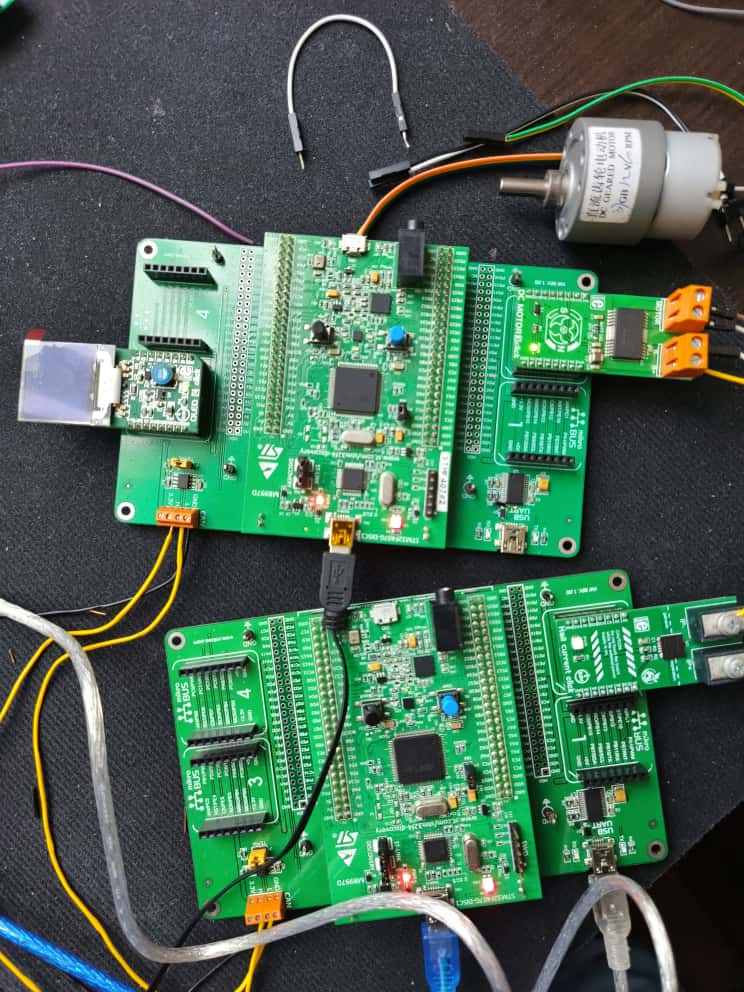
\includegraphics[width=.38\textwidth]{Resultados/Maestro_eclavo.jpg}
  \caption{Maestro y Esclavo: cableado final. Se aprecia la interfaz hacia el transceptor CAN, conexión del sensor de corriente (SPI) y UART hacia el PC.}
  \label{fig:res_maestro_cableado}
\end{figure}


\begin{figure}[H]
  \centering
  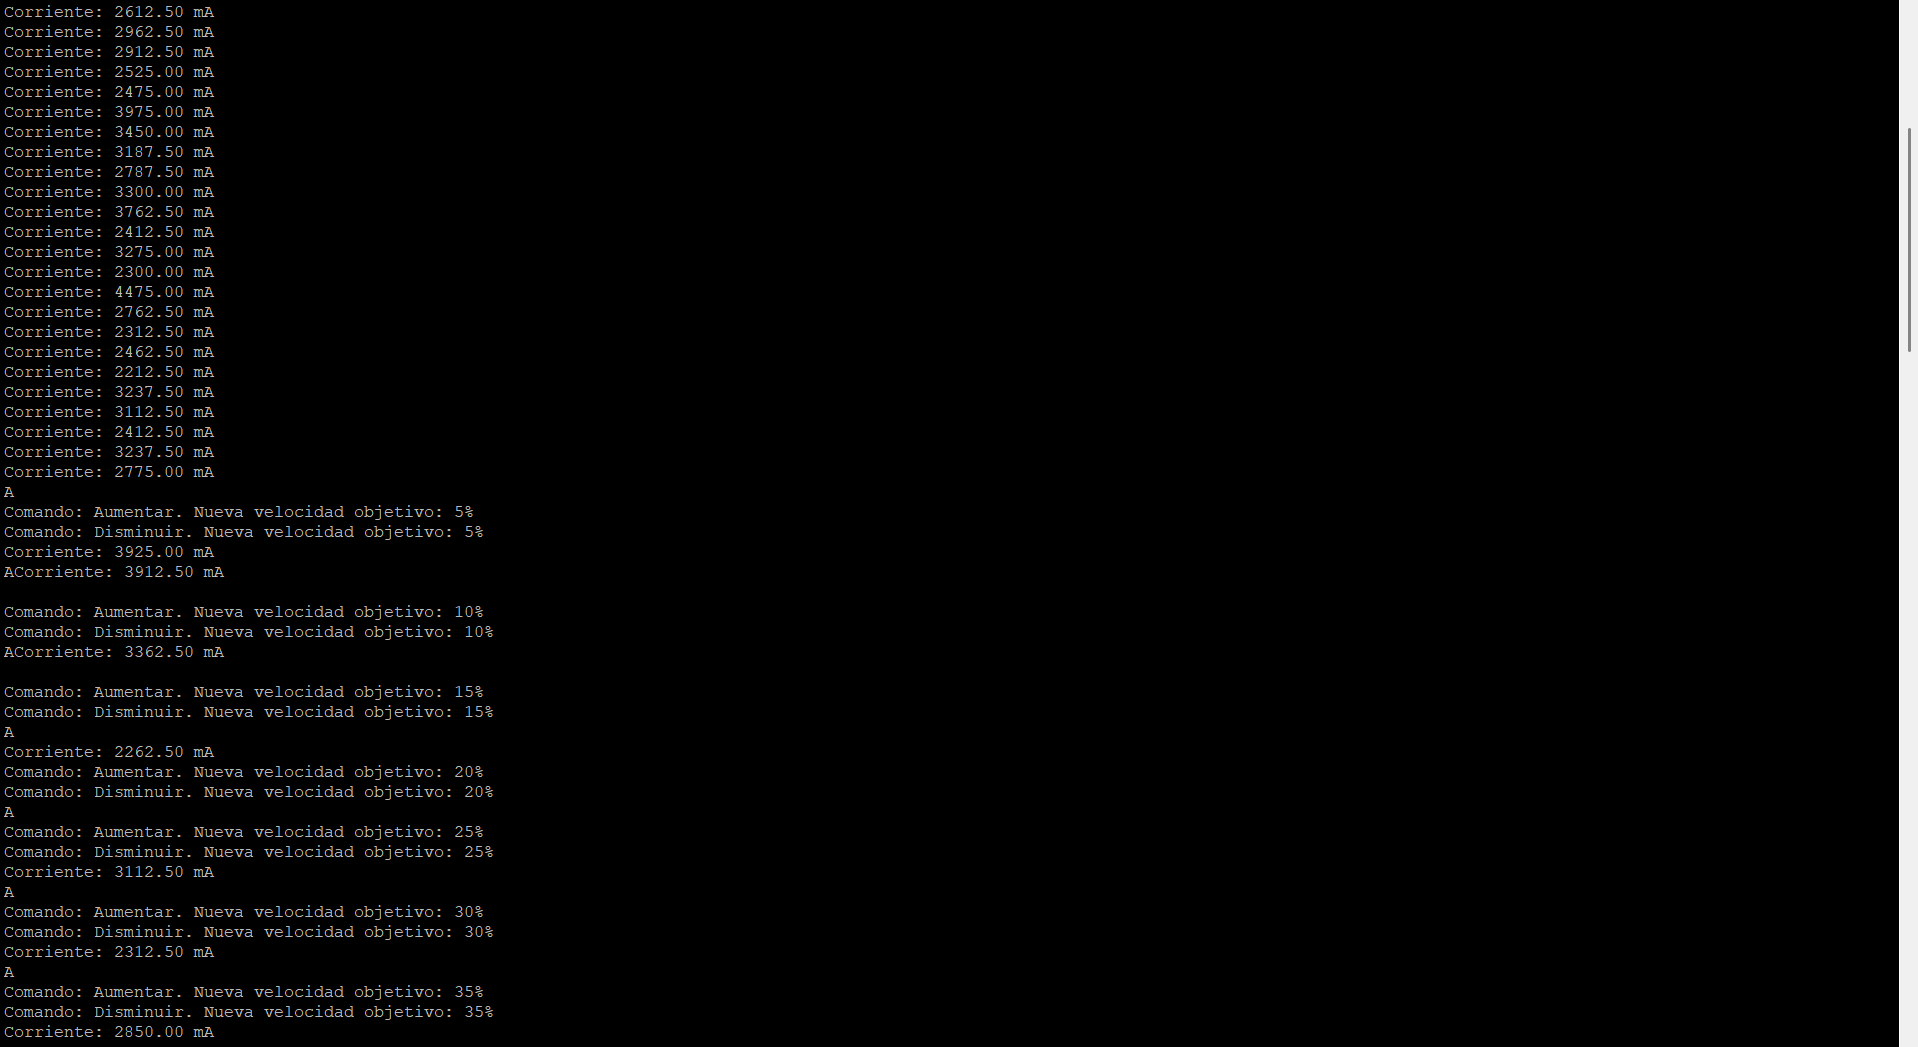
\includegraphics[width=.85\textwidth]{Resultados/Aumento.png}
  \caption{Sesión PuTTY: trazas periódicas de corriente y acuses al enviar \texttt{A/a} (sube PWM) y \texttt{D/d} (baja PWM).}
  \label{fig:res_putty_sesion}
\end{figure}

\begin{figure}[H]
  \centering
  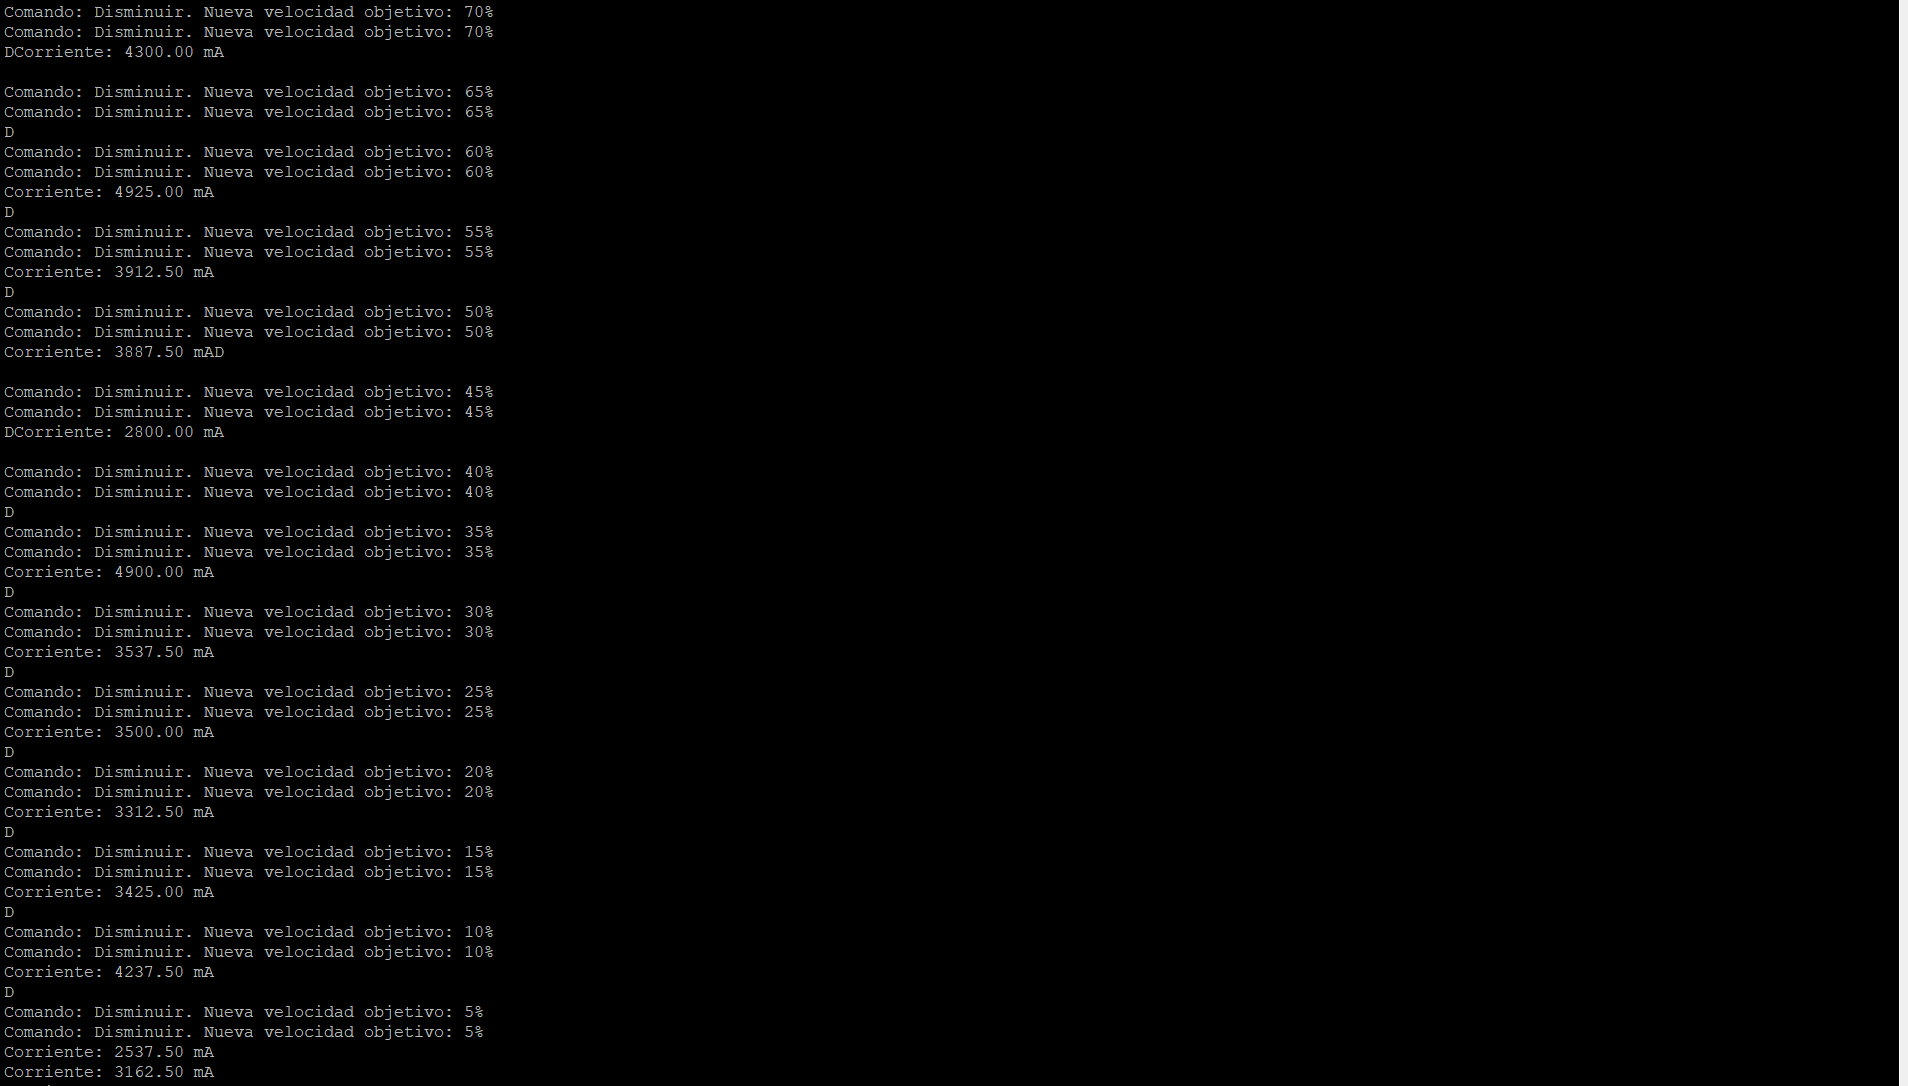
\includegraphics[width=.85\textwidth]{Resultados/Decremento.png}
  \caption{Sesión PuTTY: trazas periódicas de corriente y acuses al enviar \texttt{A/a} (sube PWM) y \texttt{D/d} (baja PWM).}
  \label{fig:res_putty_sesion}
\end{figure}






\end{document}
